%Medicinrådet beslutter efter prisforhandlingen, hvorvidt det nye lægemiddel skal anvendes som standardbehandling. Hvis dette er tilfældet foretages et kontraktskift.~\citep{Amgros2017, Amgros2017a}

%og udbud på lægemidler sker har Amgros en dialog med Medicinrådet~\citep{Amgros2017, Amgros2017a}. Lægemidlerne vurderes i forhold til effekt, eksisterende behandling og pris med det formål at stræbe efter laveste priser samt bedst mulig behandling for patienterne.~\citep{Amgros2017, Amgros2017a}

%Medicinrådet kategoriserer nye lægemidler og indikationer i forhold til den nuværende standardbehandling ud fra merværdi i stor, vigtig, lille eller ingen merværdi~\citep{Amgros2017, Amgros2017a}. Dette sammenstilles med standardbehandlingen af Amgros over en omkostningsanalyse der er udarbejdet af leverandøransøgeren for lægemidlet.
%Amgros vurderer, hvorvidt de tilsendte  oplysninger i omkostningsanalysen er relevante og valide.~\citep{Amgros2017, Amgros2017a} 

%Den kliniske merværdi, omkostningsanalysen og estimeringen af budget konsekvenser danner grundlaget for prisforhandling~\citep{Amgros2017, Amgros2017a}. Medicinrådet beslutter efter prisforhandlingen, hvorvidt det nye lægemiddel skal anvendes som standardbehandling. Hvis dette er tilfældet foretages et kontraktskift.~\citep{Amgros2017, Amgros2017a} 



%20,86~\% kliniske processor, 17,98~\% kommunikation og dokumentation samt 17,23~\% administrative processer~\citep{Patientombuddet2013}.


%Restordre kan kategoriseres som simpel eller kompleks i forhold til hvordan de påvirker klinikken~\citep{Laegemiddelinformaion2017}. En simpel restordre er vurderet til at påvirke klinikken i lav grad. Disse opstår dagligt når et lægemiddel skiftes til et simpel generisk lægemiddel og varetages ofte af sygehusapotekets logistik-afdeling. ~\citep{Laegemiddelinformaion2017}
%
%En kompleks restordre vurderes til at påvirke klinikken i mellem til høj grad ~\citep{Laegemiddelinformaion2017}. Disse sker i forbindelse med mere komplekse skift til generiske lægemidler i forbindelse med ændringer af f.eks. styrke, disponeringsform  og andre hjælpestoffer. I tilfælde af kompleks restordre henvendes der ofte kontakt til den medicinansvarlige, kontraktsygeplejersker eller medicinservicefarmakonomerne i forhold til at undersøge om lægemidlet er anvendeligt for det pågældende hospitalsafsnit. Hensigten i tilfælde af komplekse restordre er at finde en erstatning i god tid, at erstatning ligner det lægemiddel der er i restordre samt mindske ændringer ved klinikkens arbejdsgang.~\citep{Laegemiddelinformaion2017}
%
%Der udføres en faglig risikovurdering i samarbejde med sygehusapoteket og eventuelt i samarbejde klinikken ved restordre ~\citep{Laegemiddelinformaion2017}. Dette gøres med henblik på optimal lægemiddelbehandling i forhold til patientsikkerhed, ændringer i håndtering og opbevaringsbetingelser af lægemidlet. Erstatningslægemidlet vurderes ud fra prioriteringen i kategorierne registeret specialitet (RS), ikke-registeret specialist (IRS) eller magistrelt lægemiddel~\citep{Laegemiddelinformaion2017}.



%\subsection{Logistik og lægemiddelinformation}
%SRN's opgave ved udbud er at bearbejde udbudsmateriale og afgive estimater til Amgros via sygehusapoteksportalen i forbindelse med kommende kontrakter ~\citep{Sygehusapoteket2017}. De efterfølgende processer er afhængige af at materialet er gennemarbejdet og at sygehusapoteksportalen er anvendt korrekt. SRN anvender forskellige hjælpemidler ved gennemgang af Amgrosudbud, som forbrugsrapport, intern rekommandationsliste, oversigt over specialist/ATC-ansvarlige, ApoVision og Medicin.dk. ~\citep{Sygehusapoteket2017}

%Materialet gennemgås i forhold til typen af udbud af logistik og lægemiddelinformation. Hvis det er et bagatel tilbud, hvor SRN ikke er forpligtet til at acceptere dette tilbud gennemgås den økonomiske gevinst. Hvis en besparelse er tilfældet behandles materialet med henblik på skift. Der gives ikke budgettal for disse. Ved forlængelse af kontrakter gennemgås med henblik på beregning af budgettal. Ved nye udbud skal der gennemgås i forhold til budgettal, eventuelt skift og økonomi. 

%Den indsamlede information sendes videre til lægemiddelinformation og specialist/ATC-ansvarlige om kommende skift samt udbudsmateriale.

%Ved kompleks lægemiddelskift Amgrosudbud gennemgås lægemiddelskift tilsendt af amgrosansvarlig (Indkøb) som tager stilling til problemstillinger inden for egne ATC-koder.

%\subsubsection{Specialist/ATC-ansvarlige}
%Specialistfarmaceuterne er Sygehusapotekets repræsentant og tilføre farmaceutisk viden til den ATC-ansvarlige gruppe i forhold til f.eks. formuleringer, optagelse, håndtering og produktionsmæssigt. Yderligere skal sepcialisten sikre viden om økonomi, forbrug og forbrugsmønstre og kunne belyse generelle problemstillinger i forhold til rekommandationer og standardsortimenter. Sikre at problemstillinger som SRN oplever bringes videre. Problemstillinger i forhold til medicinmodulet samt sikre implementering af beslutninger, der er igangsat på specialistgruppemødet og RADS, som SRN har indflydelse på f.eks. rekommandationer, opsætningen af sagsforbehold, udarbejdelse af temanumre af lægemiddel NYT. 
%
%Fremlægger mulige fælles indsatsområder for specialistgrupper som tilhører den specifikke ATC-gruppe.
%
%
%
%


%\fxnote{\url{https://levportal.amgros.dk/SiteCollectionDocuments/1.\%20Grundl\%C3\%A6ggende\%20information\%20om\%20l\%C3\%A6gemiddeludbud.pdf}}.
 
%I disse tilfælde er sygehusapoteket ikke forpligtet til at anvende lægemidlet og leverandøren omfattes ikke af indkøbs- eller forsyningspligt.~\citep{Amgros2018}Amgros publicerer hvert år i maj/juni udbud for en række lægemidler med en mindre omsætning, der ligger under tærskelværdierne, men som kan have grænseoverskridende interesse. Derfor udbyder vi disse indkøb efter reglerne for udbud under tærskelværdierne. Det er derudover muligt for leverandører at afgive løbende tilbud på de ATC-koder, der er omfattet af bagatelkøb.

%\subsection{Typer af utilsigtede hændelser}
%\textit{Dette afsnit skal indeholde de utilsigtede hændelser der skyldes medicinering, administration og disponering. Yderligere tænker jeg at der er mulighed for at koble flere ting på ud fra den analyse som Lina foretager sig på afdelingen. Hvis det er muligt og de ikke overlapper i hinanden for meget vil jeg prøve at opdele i forhold til om det skyldes kontraktskift eller restordre.} 
%
%\subsubsection{Utilsigtede hændelser ved kontraktskift}
%De patientsikkerhedsmæssige konsekvenser opstået ved kontraktskift er undersøgt af et norsk studie~\citep{Hakonsen2010}. Interview med 100 sygeplejersker påviste at der opstod fejlmedicinering ved generiske lægemidler. Fejl i ordination og manglende dokumentation af lægemiddelskiftet foretaget af lægen blev opdaget af 46~\% sygeplejersker dagligt, hvorimod sygeplejerskerne altid fik lægemiddelsiftet dokumenteret. Yderligere følte 92~\% af sygeplejerskerne at generiske lægemidler var tidskrævende og 91~\% at disse øgede risikoen for fejl ved disponering.~\citep{Hakonsen2010}. De typiske hændelser ved kontraktskift fremgår af Figur \ref{fig:UTHkontraktskift}.
%
%\begin{figure}[H]\centering
%	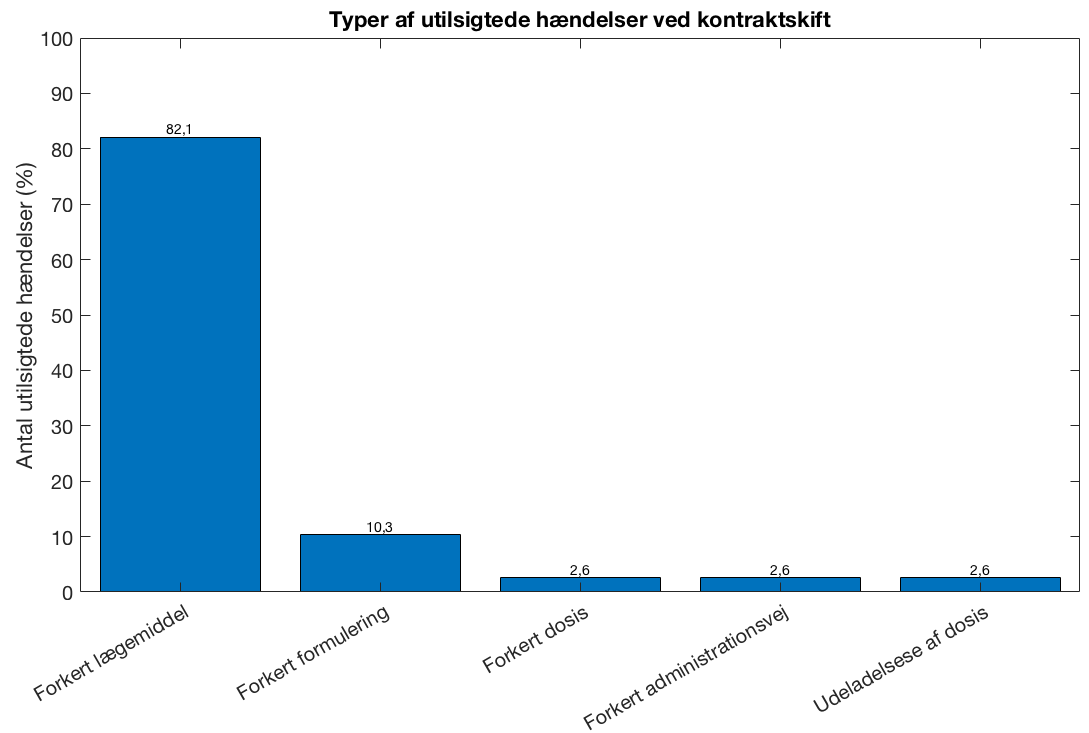
\includegraphics[width=0.7\textwidth]{billeder/UTH1.png} 
%	\caption{Utilsigtede hændelser opstået ved kontraktskift\citep{Hakonsen2010}.}
%	\label{fig:UTHkontraktskift}  
%\end{figure}
%
%Af Figur \ref{fig:UTHkontraktskift} fremgår det at 82,1~\% af UTH'erne forekommer ved disponering af forkert lægemiddel. Den næst hyppigste er forkert formulering hvor 10,3\% af UTH'er er berettiget mod dette. I  sjældnere tilfælde sker forkert dosis, administrationsvej samt udeladelse af dosis. 




%\subsubsection{Utilsigtede hændelser ved restordre}
%***  Dette afsnit skal ligne afsnittet omkring kontraktskift ***

%*** KIG 3.5.5. Utilsigtede hændelser forårsaget af Restordre *** 16 PDF
%
%De typiske hændelser ved restordre fremgår af Figur \ref{fig:UTHrestordre}.
%
%\begin{figure}[H]\centering
%	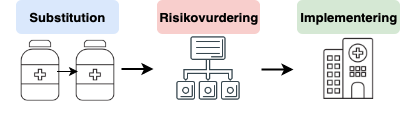
\includegraphics[width=1\textwidth]{billeder/forside.png} 
%	\caption{Utilsigtede hændelser opstået ved restordre\citep{Hakonsen2010}.}
%	\label{fig:UTHRestordre}  
%\end{figure}



Siden år 2007 har Amgros sendt lægemidler i udbud med henblik på at indkøbe lægemidler af højkvalitet med mest mulig besparelse til de offentlige danske hospitaler, hvilket har medført en besparelse på 3,1 millarder kroner i år 2017~\citep{Amgros2017b}. Et udbud kan forekomme hvis der findes mere end én leverandør af lægemidlet. I tilfælde af patent på et lægemiddel, hvormed der kun findes én leverandør, sættes lægemidlet sjældent i konkurrence, da prisen allerede er fastsat.~\citep{Amgros2015}.

Størstedelen af udbud på lægemidler i ATC-grupper sker en gang årligt fra start september til midt november, det så kaldte Amgrosudbud\citep{Sygehusapoteket2017}. Hvor mindre udbud sker løbende hen over året og omfatter udbud på ATC-grupper som indgår i Medicinrådet behandlingsvejledninger.\citep{Sygehusapoteket2017, Danskeregioner}. 